\section{Transformaciones de variables}
\label{sec:transformaciones}

El análisis distribucional presentado en la Sección~\ref{sec:analisis_distribucional} 
mostró que varias variables presentan distribuciones asimétricas. Dado que estas 
variables se incorporan como predictores de un modelo lineal, resulta relevante 
evaluar si una representación más simétrica mejora su capacidad para explicar la 
señal EEG. Con este objetivo, se exploraron dos transformaciones. La primera es 
el logaritmo natural:

%
\begin{equation}
    f(x) = \log(x)
\end{equation}
%
cuya aplicación se justifica para variables con distribuciones de cola 
larga, ya que contrae los valores extremos y reduce el sesgo a la derecha. 
La segunda es la transformación logit:
%
\begin{equation}
    f(x) = \log\left(\frac{x}{1-x}\right)
\end{equation}
%
que se aplica a variables acotadas en el intervalo $(0,1)$, llevándolas 
al espacio real $(-\infty, +\infty)$, lo cual es teóricamente más apropiado 
para su uso como predictor en un modelo lineal.

Las transformaciones exploradas para cada variable se resumen en la 
Tabla~\ref{tab:transformaciones}. La elección de cada transformación 
estuvo guiada por las características distribucionales observadas en 
la Sección~\ref{sec:analisis_distribucional}. A continuación se detalla 
el análisis particular de cada variable.

\begin{table}[H]
\centering
\label{tab:transformaciones}
\begin{tabular}{p{3.5cm}p{4.5cm}p{4.5cm}}
\toprule
\textbf{Categoría} & \textbf{Variable} & \textbf{Transformaciones} \\
\midrule
\multirow{2}{*}{Bottom-up} 
  & \feat{saliencia\_pixel}      & $\log(x)$ \\
  & \feat{saliencia\_media}      & $\log(x)$ \\
\midrule
\multirow{2}{*}{Similitud con el target} 
  & \feat{similitud\_pixel}      & $\log(x)$ \\
  & \feat{similitud\_media}      & $\log(x)$ \\
\midrule
\multirow{2}{*}{\parbox{3.5cm}{Estado interno del\\proceso bayesiano}} 
  & \feat{ganancia\_informacion} & $\log(x)$ \\
  & \feat{posterior}             & $\log(x)$, logit$(x)$ \\
\midrule
\multirow{2}{*}{Calidad de la decisión} 
  & \feat{gap\_entropia}         & $\log(x)$ \\
  & \feat{distancia\_grilla}     & $\log(x)$ \\
\midrule
\multirow{2}{*}{\parbox{3.5cm}{Competencia entre\\candidatos}}
  & \feat{competencia\_densidad} & $\log(x)$ \\
  & \feat{competencia\_fp\_max}  & $\log(x)$ \\
\bottomrule
\end{tabular}
\caption{Transformaciones exploradas por variable.}
\end{table}

\subsubsection{Transformaciones a variables Bottom-Up}

Para las variables \feat{saliencia\_media} y \feat{saliencia\_pixel} la aplicación de $\log(x)$ redujo la asimetría para ambos casos. Para \feat{saliencia\_media} la distribución resultante 
es aproximadamente simétrica y unimodal. 

\begin{figure}[H]
    \centering
    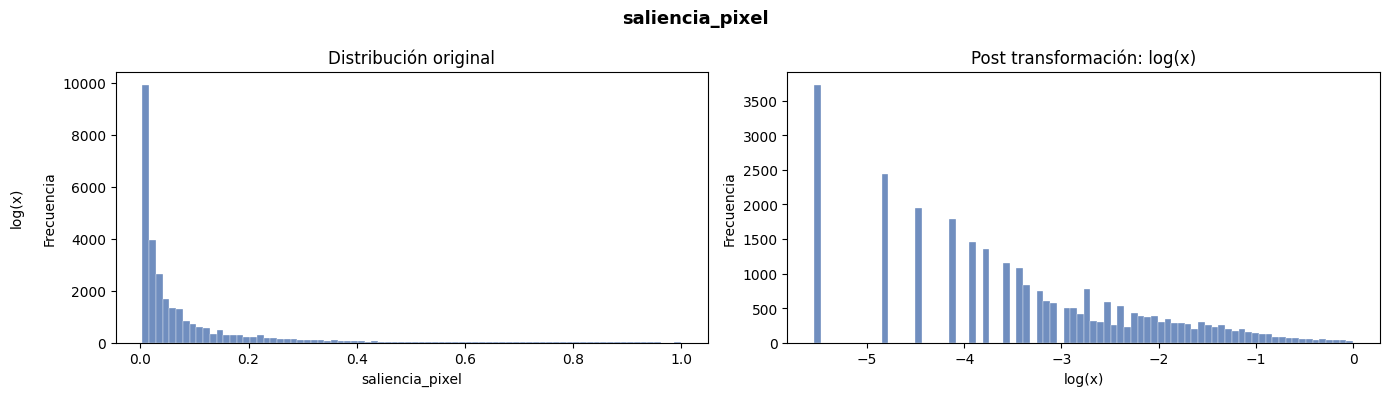
\includegraphics[width=\textwidth]{chapters/04_extraccion_analisis_variables/images/transf_saliencia_pixel}
    \caption{Distribución de la variable saliencia\_pixel transformada}
    \label{fig:transf_saliencia_pixel}
\end{figure}

En el caso de \feat{saliencia\_pixel} 
la transformación también reduce la asimetría, aunque la distribución 
resultante presenta una estructura multimodal con picos discretos.  
Esto es consistente con la naturaleza puntual de esta variable: 
\feat{saliencia\_pixel} toma el valor en 
el píxel exacto de fijación, lo que introduce mayor variabilidad 
y concentración en valores específicos.

\begin{figure}[H]
    \centering
    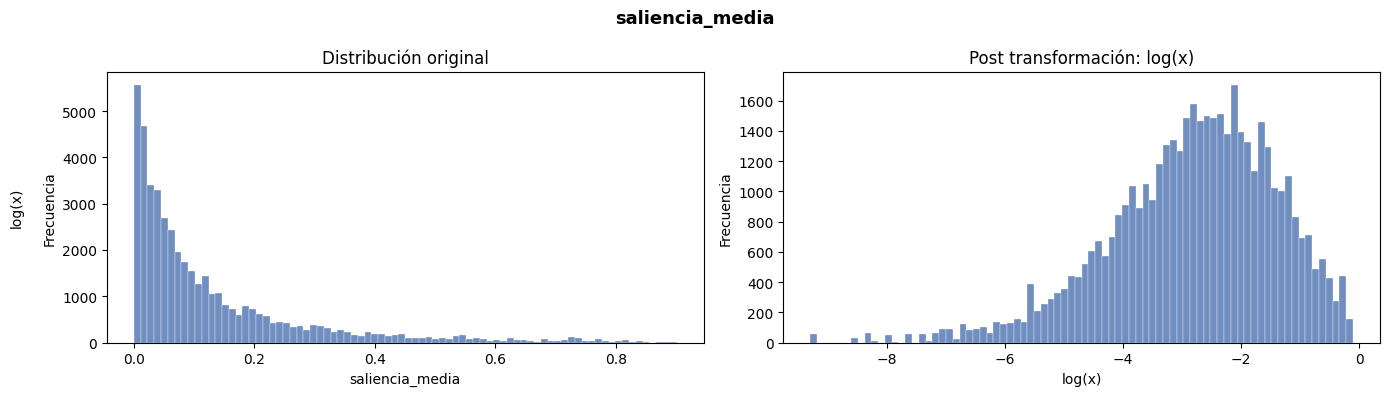
\includegraphics[width=\textwidth]{chapters/04_extraccion_analisis_variables/images/transf_saliencia_media.png}
    \caption{Distribución de la variable saliencia\_media transformada}
    \label{fig:transf_saliencia_media}
\end{figure}

\subsubsection{Transformaciones a variables de Similitud con el target}

Las variables \feat{similitud\_media} y \feat{similitud\_pixel} presentan 
distribuciones análogas a las observadas en las 
variables bottom-up. La aplicación de $\log(x)$ produce resultados 
similares en ambos casos: en \feat{similitud\_media} la distribución 
resultante es aproximadamente simétrica y unimodal, mientras que en 
\feat{similitud\_pixel} la distribución resultante mantiene cierta irregularidad con picos 
discretos, consistente con su naturaleza puntual.

\begin{figure}[H]
    \centering
    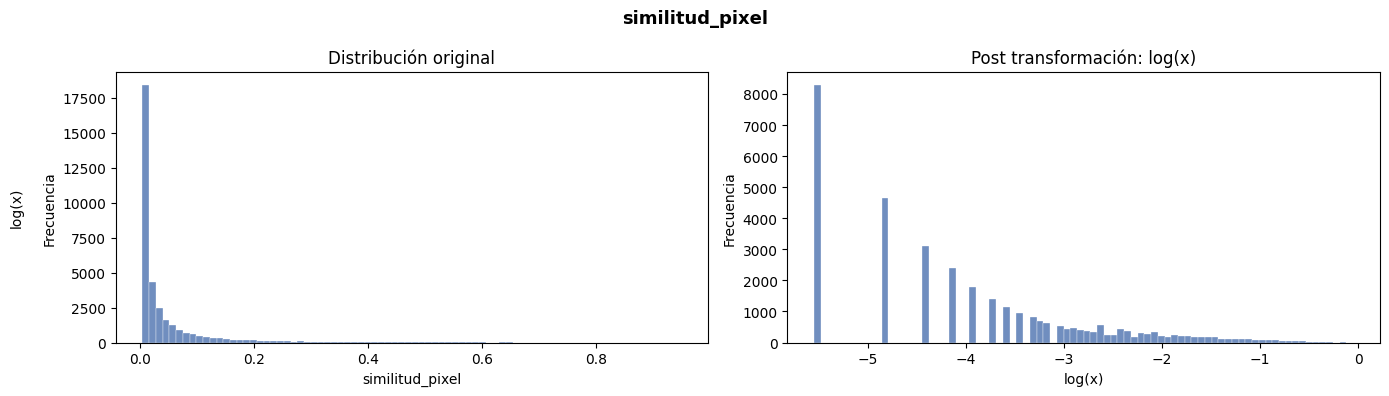
\includegraphics[width=\textwidth]{chapters/04_extraccion_analisis_variables/images/transf_similitud_pixel.png}
    \caption{Distribución de la variable similitud\_pixel transformada}
    \label{fig:transf_similitud_pixel}
\end{figure}.

\begin{figure}[H]
    \centering
    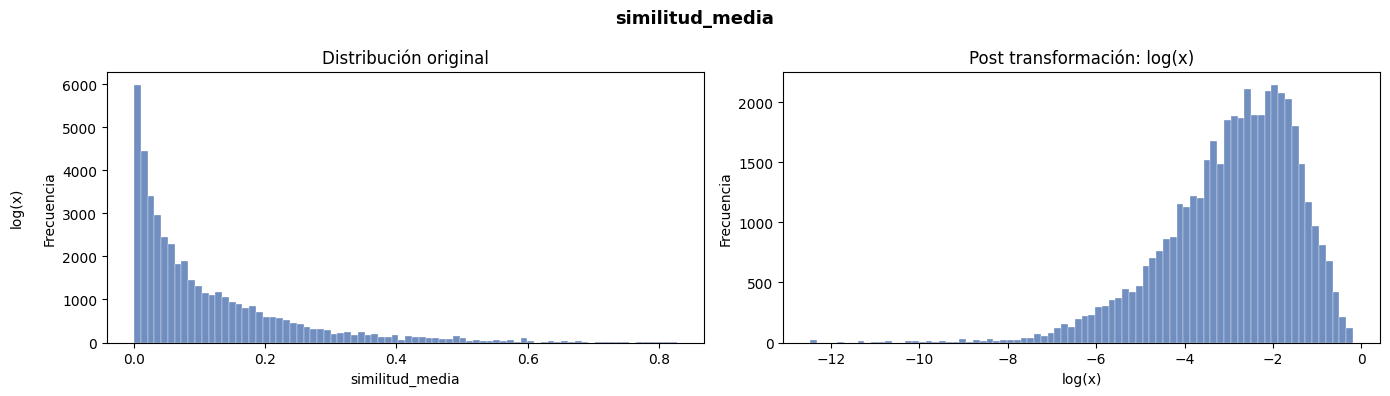
\includegraphics[width=\textwidth]{chapters/04_extraccion_analisis_variables/images/transf_similitud_media.png}
    \caption{Distribución de la variable similitud\_media transformada}
    \label{fig:transf_similitud_media}
\end{figure}.

\subsubsection{Transformaciones a variables de Estado interno del proceso bayesiano}

La aplicación de $\log(x)$ resuelve la asimetría de \feat{ganancia\_informacion} de forma efectiva, produciendo 
una distribución aproximadamente simétrica y unimodal.

\begin{figure}[H]
    \centering
    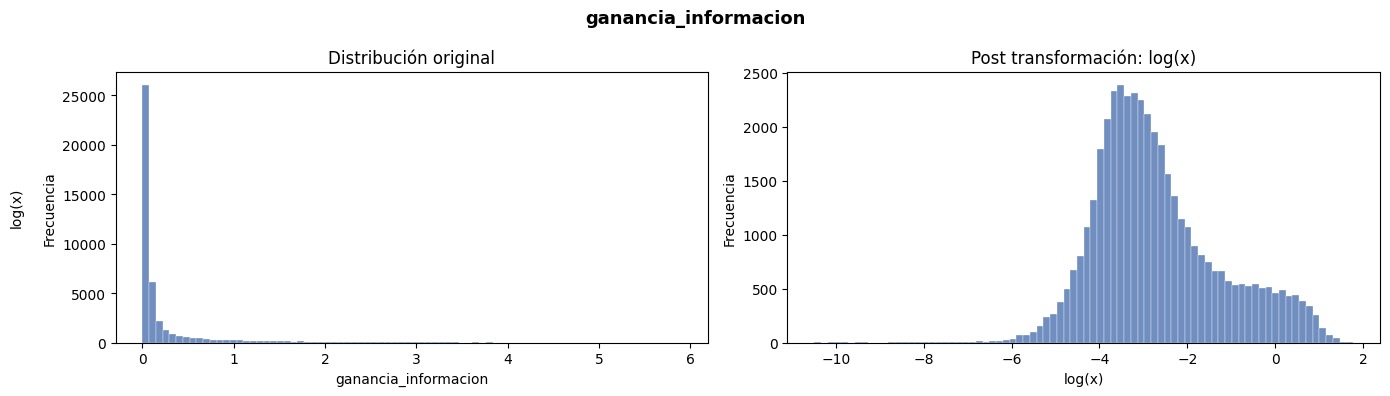
\includegraphics[width=\textwidth]{chapters/04_extraccion_analisis_variables/images/transf_ganancia_informacion.png}
    \caption{Distribución de la variable ganancia\_información transformada}
    \label{fig:transf_ganancia_informacion}
\end{figure}

Se exploraron dos transformaciones para la variable \feat{posterior}: la transformación 
$\log(x)$ produce una distribución aproximadamente simétrica y unimodal, 
reduciendo efectivamente la asimetría original; la transformación logit produce 
un resultado distribucional similar.


\begin{figure}[H]
    \centering
    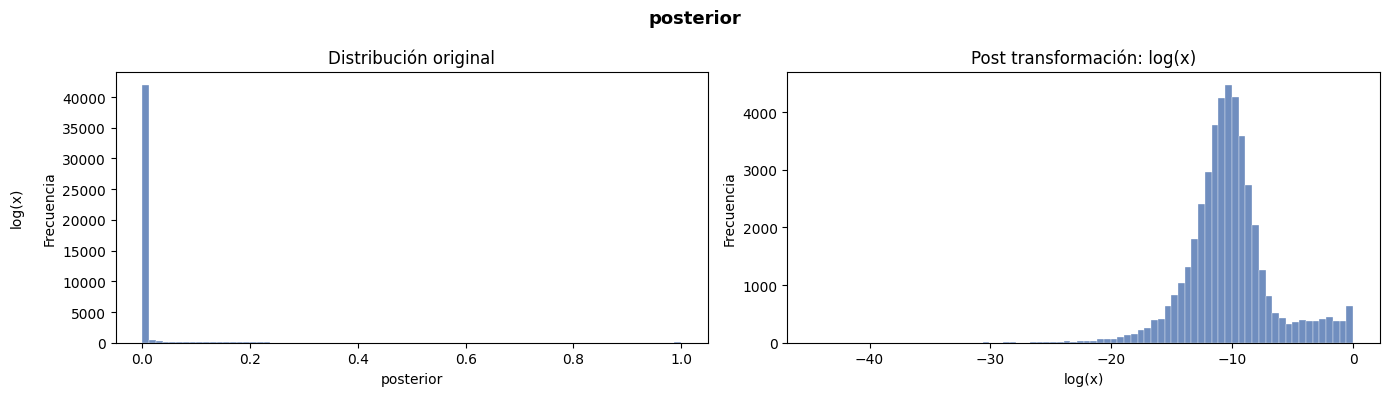
\includegraphics[width=\textwidth]{chapters/04_extraccion_analisis_variables/images/transf_posterior_log.png}
    \caption{Distribución de la variable posterior transformada}
    \label{fig:transf_posterior_log}
\end{figure}

\begin{figure}[H]
    \centering
    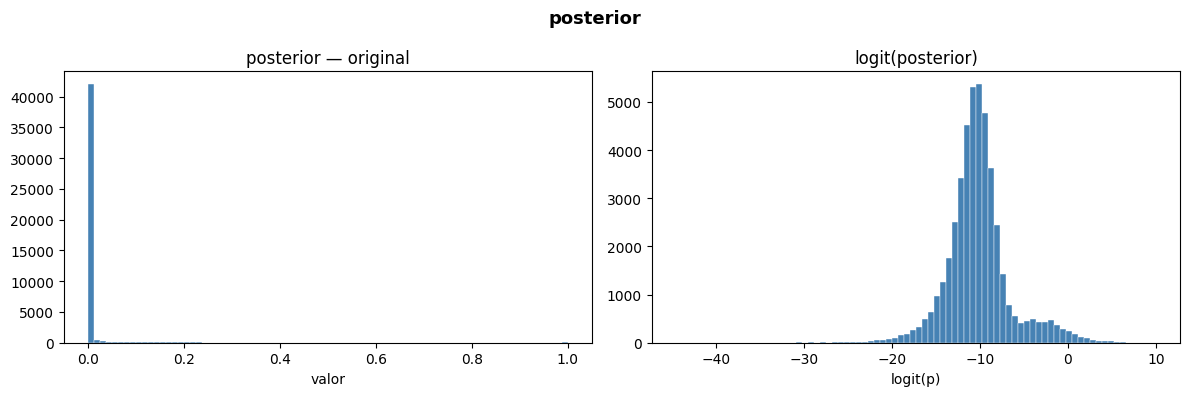
\includegraphics[width=\textwidth]{chapters/04_extraccion_analisis_variables/images/transf_posterior_logit.png}
    \caption{Distribución de la variable posterior transformada}
    \label{fig:transf_posterior_log}
\end{figure}


\subsubsection{Transformaciones a variables de Calidad de la decisión}

La aplicación de $\log(x)$ mejora 
la simetría de la distribución de \feat{gap\_entropia}, produciendo una forma aproximadamente unimodal, 
aunque persiste una leve asimetría en la cola derecha.

\begin{figure}[H]
    \centering
    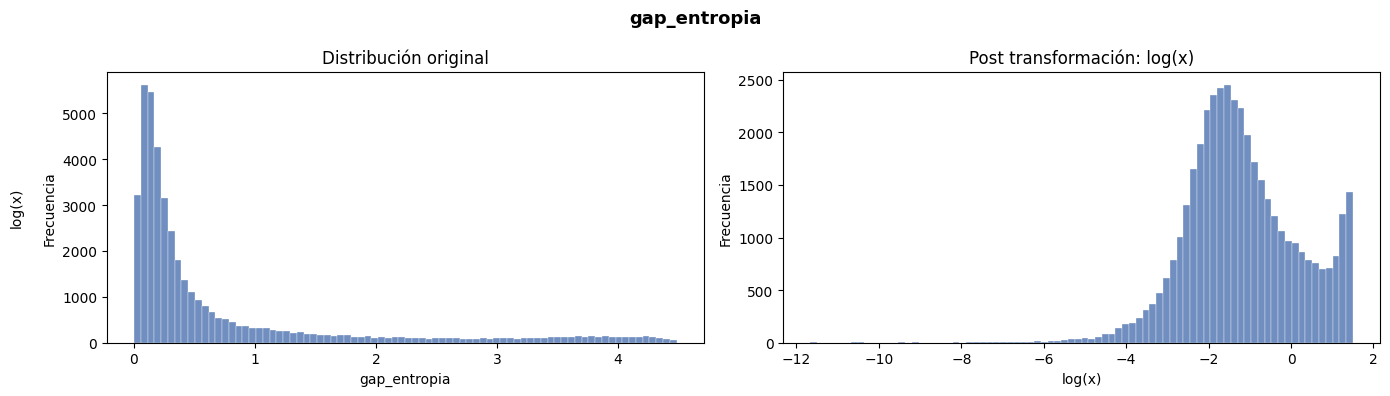
\includegraphics[width=\textwidth]{chapters/04_extraccion_analisis_variables/images/transf_gap_entropia.png}
    \caption{Distribución de la variable gap\_entropia transformada}
    \label{fig:transf_gap_entropia}
\end{figure}


La variable \feat{distancia\_grilla} presenta un comportamiento distinto al 
resto de las variables analizadas. Su distribución original muestra una estructura 
multimodal con picos discretos, lo cual es esperable dado que esta variable 
toma valores enteros que representan distancias en celdas. La aplicación 
de $\log(x)$ no resuelve esta irregularidad: la distribución transformada 
mantiene la misma estructura discreta, dado que la transformación logarítmica 
preserva el orden y la separación entre valores enteros consecutivos.

\begin{figure}[H]
    \centering
    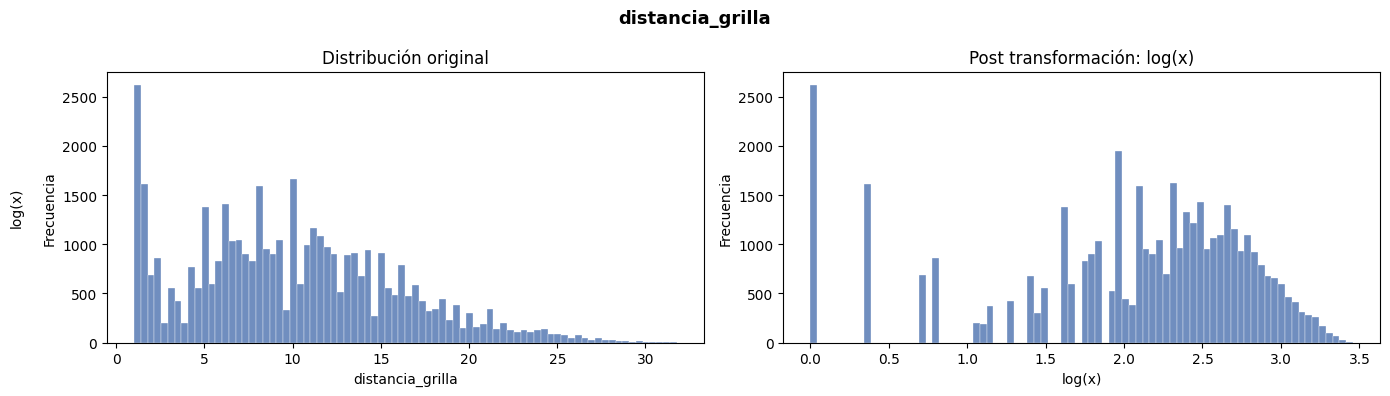
\includegraphics[width=\textwidth]{chapters/04_extraccion_analisis_variables/images/transf_distancia_grilla.png}
    \caption{Distribución de la variable distancia\_grilla transformada}
    \label{fig:transf_distancia_grilla}
\end{figure}

\subsubsection{Transformaciones a variables de Competencia entre candidatos}

A diferencia de los casos anteriores, la aplicación de $\log(x)$ no resuelve la asimetría 
en la distribución de \feat{competencia\_densidad}: la distribución transformada mantiene una estructura irregular 
dominada por pocos valores discretos, lo que sugiere que esta variable no se 
beneficia de una transformación logarítmica.

\begin{figure}[H]
    \centering
    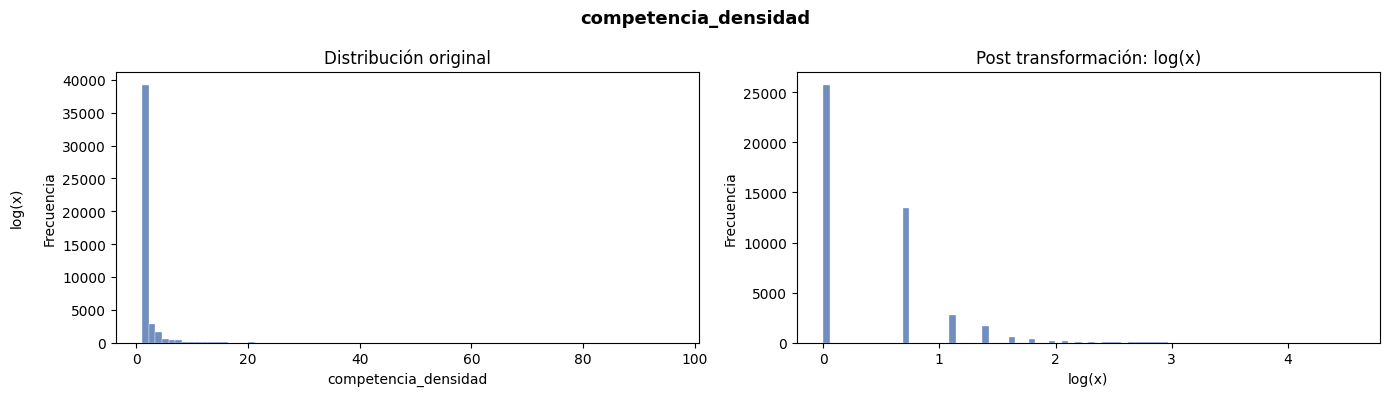
\includegraphics[width=\textwidth]{chapters/04_extraccion_analisis_variables/images/transf_competencia_densidad.png}
    \caption{Distribución de la variable competencia\_densidad transformada}
    \label{fig:transf_competencia_densidad}
\end{figure}

La aplicación de 
$\log(x)$ mejora considerablemente la simetría de la distribución de \feat{competencia\_fp\_max}, produciendo una forma 
más simétrica, aunque persiste una leve asimetría a la izquierda y un pico 
aislado en el extremo derecho.

\begin{figure}[H]
    \centering
    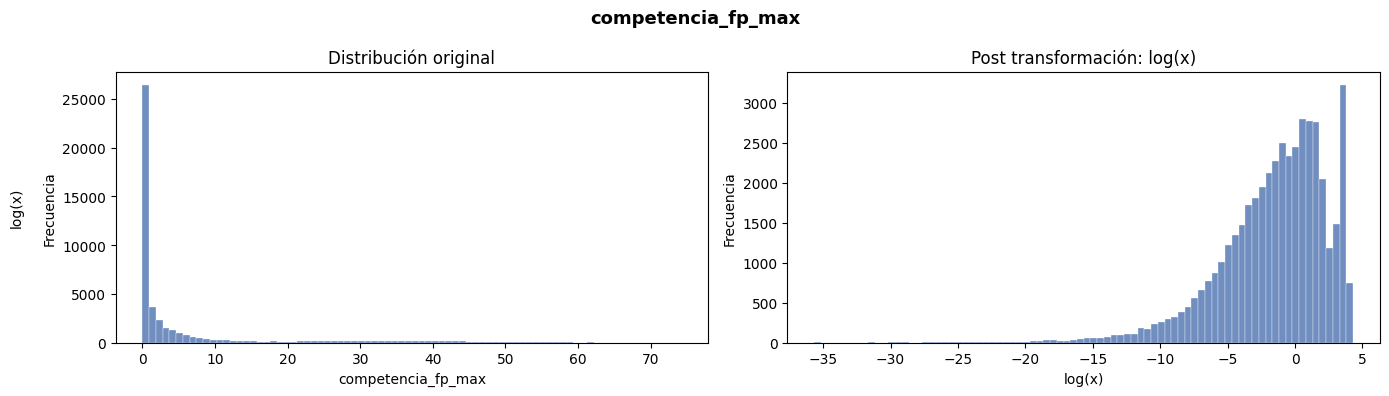
\includegraphics[width=\textwidth]{chapters/04_extraccion_analisis_variables/images/transf_competencia_fp_max.png}
    \caption{Distribución de la variable competencia\_fp\_max transformada}
    \label{fig:transf_competencia_fp_max}
\end{figure}